\subsection{The Format Inference Engine}
\label{sec:inference}

Although writing data specifications in a high-level language like
\pads{} can make managing ad hoc data much easier,
the problem of producing the description in the first place
remains. Writing such descriptions can be tedious and time consuming,
often requiring iteration. The first part of the process usually
involves an analyst writing a description of as
much of the data as they understand. From this description, the analyst
might generate and run analysis tools to find any unknown parts of the
data. He or she then studies those unknown parts of the data and refines the description
accordingly.   The process repeats until all the data can be processed successfully.
Naturally, the larger and more varied the data, the more time-consuming,
error-prone and difficult the process.  Having a tool to help produce such 
descriptions automatically would dramatically speed up construction of
network monitoring systems and subsystems and quickly allow for easy inclusion of
new or evolving data types into existing infrastructure.


% \begin{floatingfigure}[r]{3.5in}

% \hspace{4mm}
% 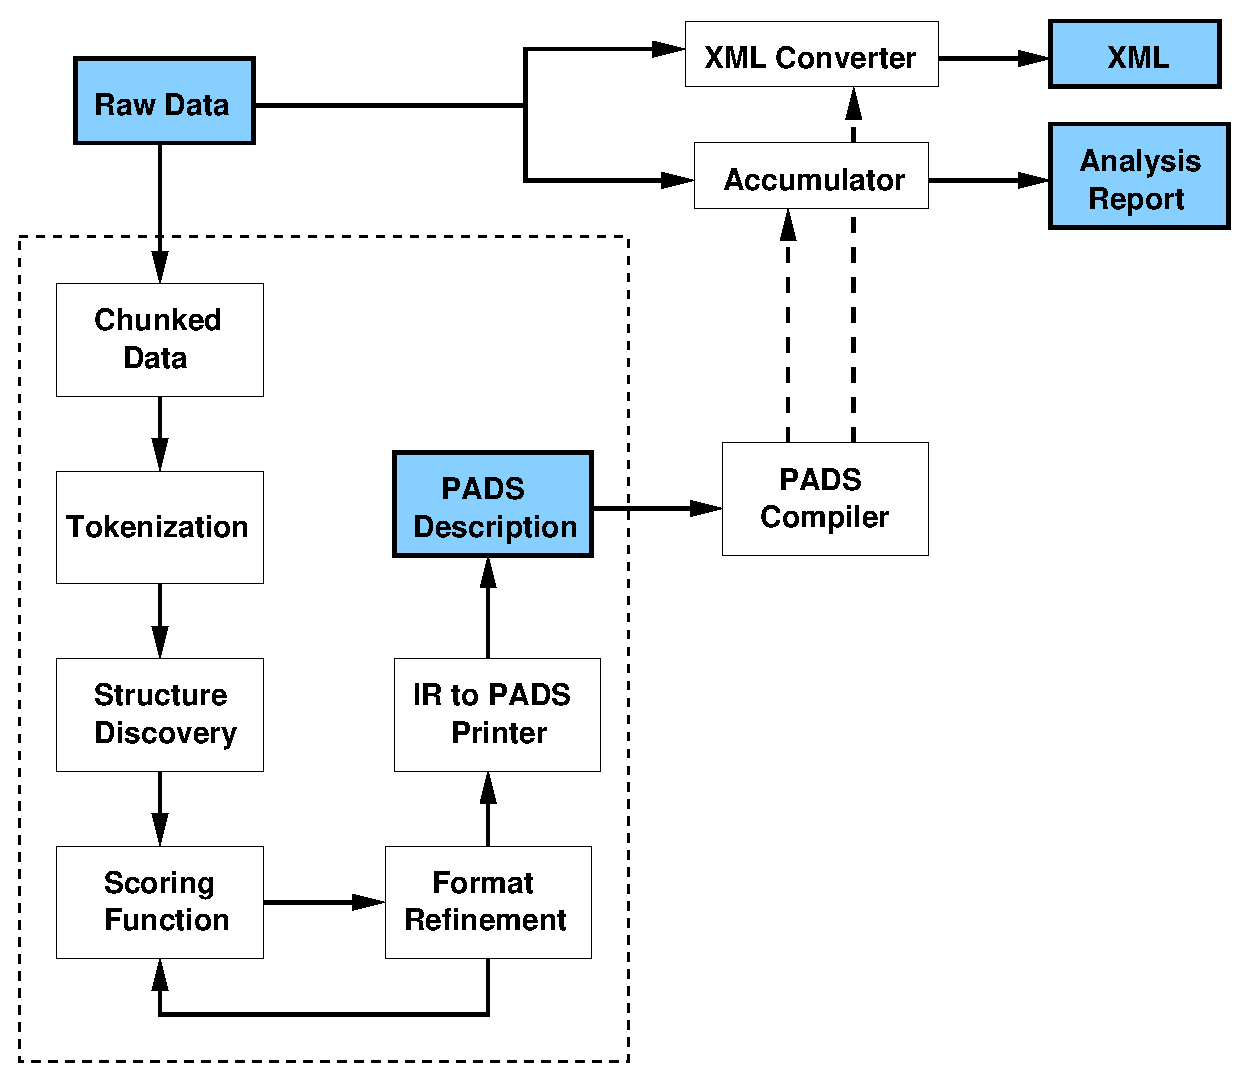
\psfig{file=format-inference-engine.eps,width=3in}
% %\includegraphics{dave.jpg}
% %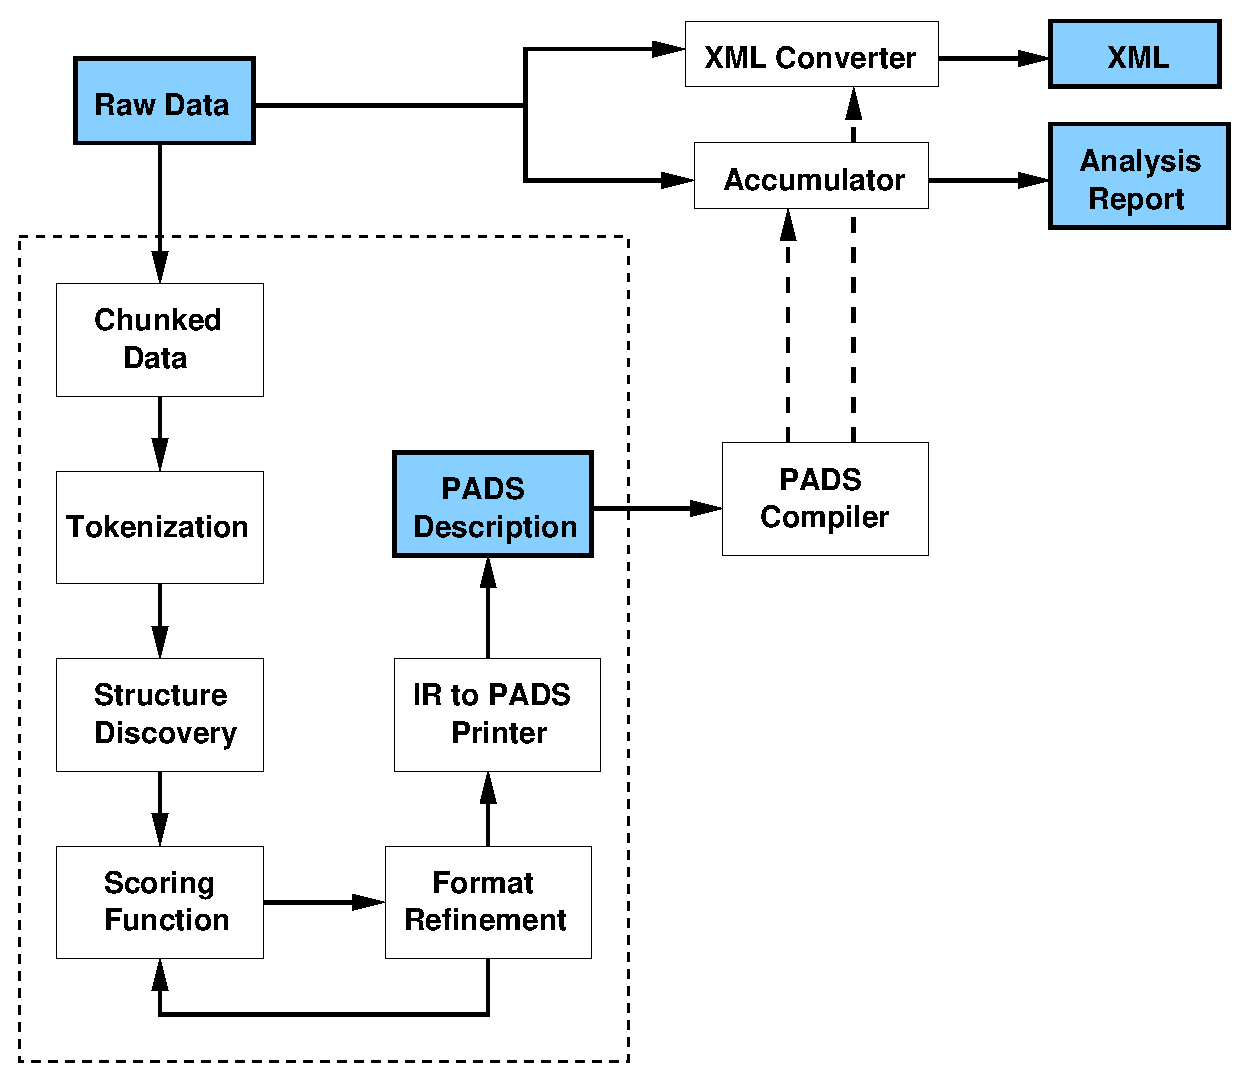
\psfig{file=format-inference-engine.eps,width=4in}
% \caption{fig:default}
% \label{fig:figlabel}
% \end{floatingfigure}

% 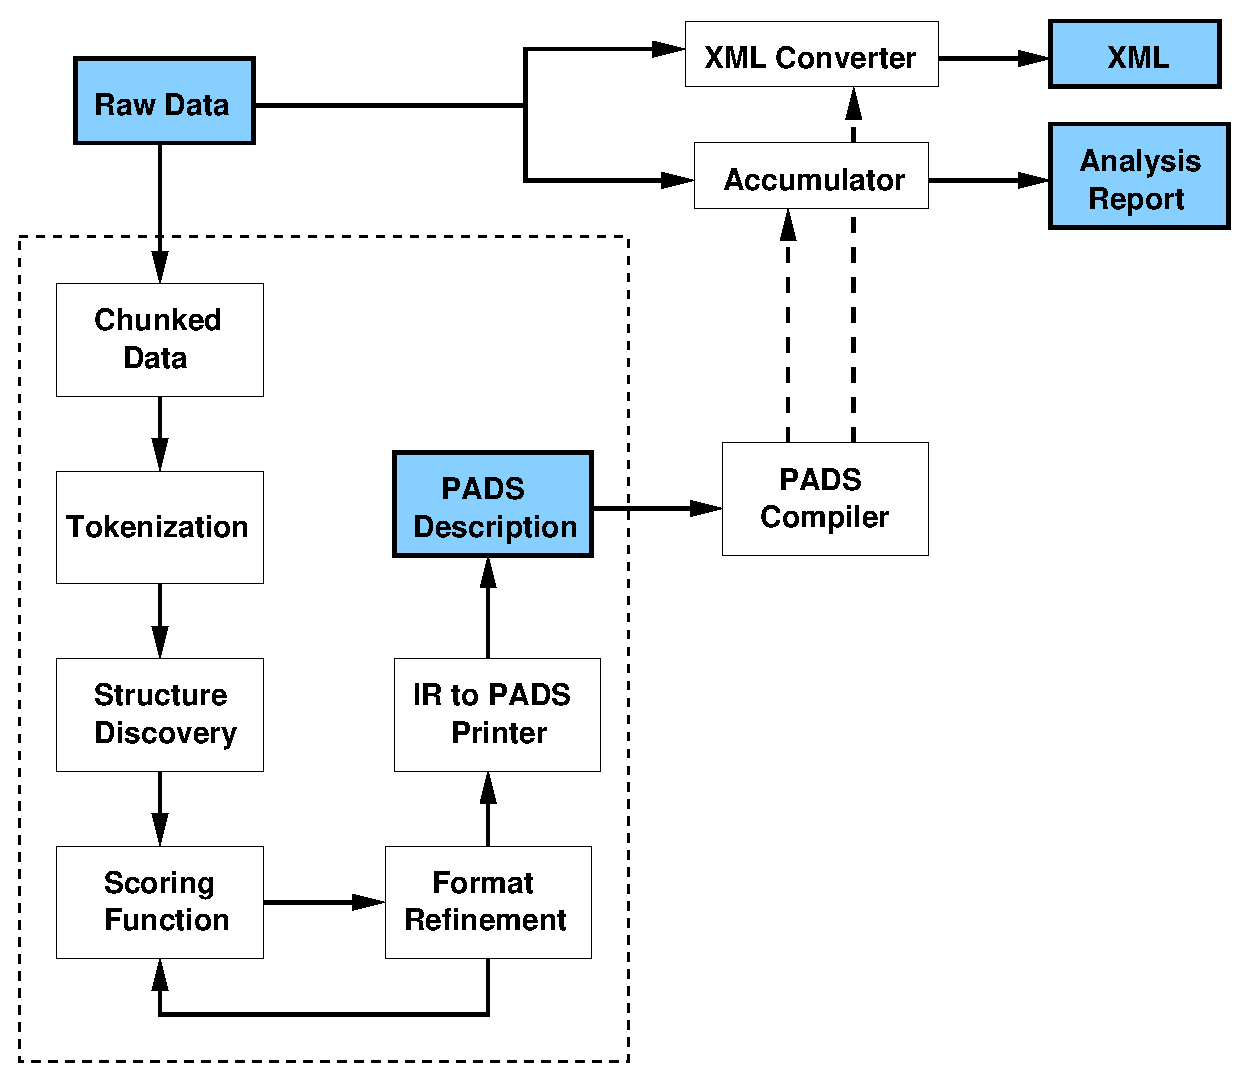
\psfig{file=format-inference-engine.eps,width=3in}


In preparation for this proposal and as an initial test of the
feasibility of our ideas, we have begun to build a tool for automatic
format inference~\cite{Fisher+:dirttoshovels}.  The following paragraphs explain the architecture
of our system and proposed research on this task.

\paragraph*{Algorithms and Architecture for Format Inference.}
The heart of the proposal involves the development of a highly modular, multi-phase
format inference engine for application log files.  These phases include:

\begin{itemize}
\item {\bf Chunking:}  Partition the data (either line-by-line,
  paragraph-by-paragraph, or file-by-file) into chunks with similar structure.
\item {\bf Tokenization:}  Convert each chunk of data into a list of 
{\em tokens} such as numbers, words, punctuation, dates, times, IP addresses, phone numbers, etc.
\item {\bf Structure Discovery:}  Use statistical analysis of token
  frequencies to produce a {\em candidate format} --- a good ``guess''
  as to what the optimal format may look like. 
\item {\bf Format Scoring and Optimization:}  Score the format
  according to a metric that measures how how compact and descriptive
  it is.  Repeatedly apply a set of rewriting rules that reduce the
  metric until no such rules exist.
\end{itemize}

We assume that the user specifies how to do chunking.  However,
tokenization, structure discovery and format scoring and optimization are all
fully automated.  Developing effective algorithms for these phases so they together 
produce compact, human-readable descriptions requires much research. 

\paragraph*{Scaling to Large Data Sets.}  Learning the format of a large
log file all at once is infeasible.  Hence, even if we discover perfect
algorithms for tokenization, structure discovery and format scoring and optimization
on small files, we require additional research to apply these algorithms
to realistic log files of large size.  We believe the key to doing so is to invent
new {\em incremental} versions of our algorithms capable of 
processing large files by iteratively applying more expensive
algorithms on small, manageable chunks.  The research challenges
involved in this endeavor include (1) techniques for summarizing
information discovered in one small chunk and passing it on to the
next, (2) techniques for effectively and
efficiently merging the results of format inference on small chunks
to create an overall description, and (3) analyzing the complexity and
improving the efficiency of existing algorithms.

\paragraph*{Global Archive Inference.}  Our initial prototype inference algorithm
was designed for determining the structure of a single log file.
However, a single application will often generate multiple different
sorts of logs -- for performance monitoring, for debugging, for 
historical analysis and for exceptional circumstances.  Moreover,
sets of applications will create sets of logs.  All of these logs
will be organized in repositories spanning multiple directories.
Hence, we will also need to explore new techniques for analyzing the contents
of entire directories and their subdirectories.  Our new techniques
will seek to explain the structure of a repository and present it graphically
to the user for further analysis and mining.